\section{Apache Spark}

\subsection{Overview}

Apache Spark is a unified, open-source analytics engine for large-scale data processing,
originally developed at UC Berkeley's AMPLab in 2009 and donated to the Apache Software
Foundation in 2010.
Its central design goal is a \emph{single programming model} — the DataFrame / Dataset API — that
executes identically for batch jobs, streaming queries, machine-learning workloads (MLlib),
and graph analytics (GraphX).

\begin{figure}[H]
  \centering
  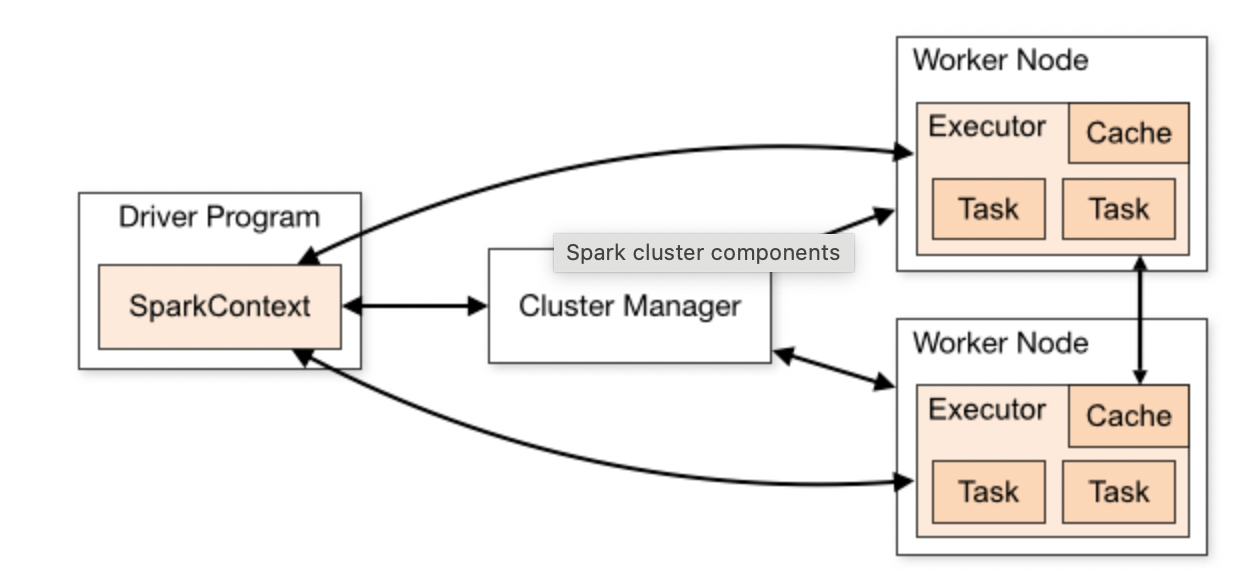
\includegraphics[width=0.88\textwidth]{image/engine/spark_architecture.png}
  \caption{Apache Spark cluster architecture: Driver, Cluster Manager, and Executors.}
  \label{fig:spark-arch}
\end{figure}

Key internal components that make Spark fast:
\begin{itemize}
  \item \textbf{Catalyst optimiser} — a rule-based and cost-based query planner that rewrites
        logical plans into optimal physical plans. It applies predicate pushdown, constant folding,
        join reordering, and many other transformations automatically.
  \item \textbf{Tungsten execution engine} — replaces JVM object representation with binary,
        off-heap memory layout and generates whole-stage bytecode at runtime (code generation),
        achieving near-native CPU efficiency.
  \item \textbf{RDD (Resilient Distributed Dataset)} — the foundational fault-tolerant abstraction.
        An RDD is a partitioned collection of records with a lineage graph that allows any lost
        partition to be recomputed from its parent RDDs. DataFrames and Datasets are typed views
        built on top of RDDs.
\end{itemize}

\subsection{Spark Streaming: Micro-batch and Real-time Mode}

Spark Structured Streaming extends the DataFrame API to unbounded data streams.
The key insight is that a stream is treated as a \emph{continuously appended, unbounded table}:
each new trigger appends new rows, and the query always returns the same DataFrame-style result.

\subsubsection{Micro-batch Mode}

\begin{figure}[H]
  \centering
  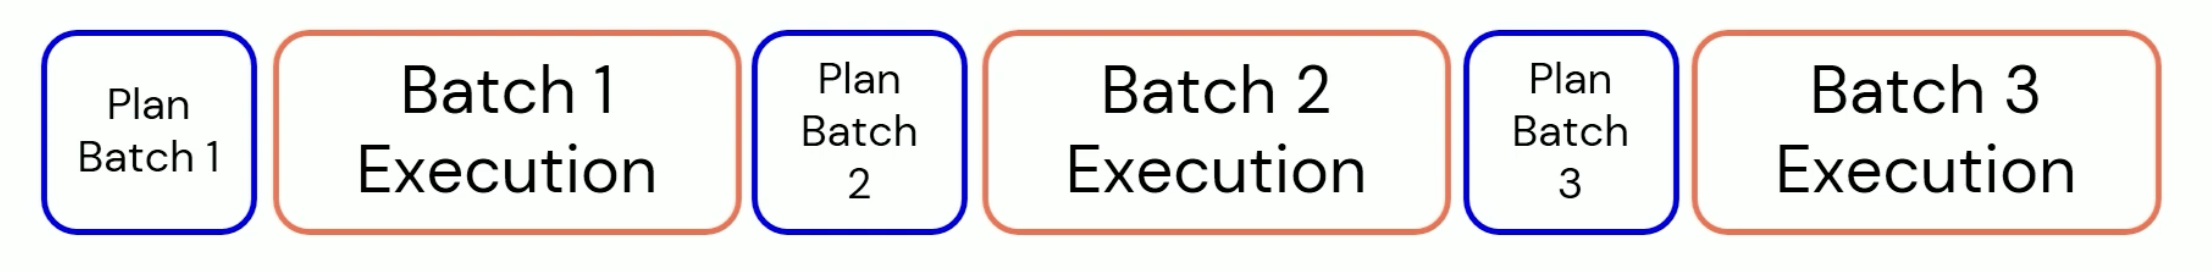
\includegraphics[width=0.88\textwidth]{image/engine/spark_micro_batch.png}
  \caption{Spark Structured Streaming micro-batch execution model.}
  \label{fig:spark-microbatch}
\end{figure}

In micro-batch mode (the default), the driver divides time into discrete \emph{trigger intervals}
and processes all records that arrived in each interval as a single bounded batch:

\begin{enumerate}
  \item The driver queries the source (e.g.\ Kafka) for new offsets since the previous trigger.
  \item It constructs a bounded DataFrame containing those records (the \emph{micro-batch}).
  \item Catalyst optimises the query plan and Tungsten executes it across the Executor pool.
  \item Results are written to the sink; source offsets are committed to the checkpoint store.
  \item After the configured \textbf{trigger interval} (e.g.\ \texttt{processingTime="5 seconds"}),
        the cycle repeats.
\end{enumerate}

\begin{figure}[H]
  \centering
  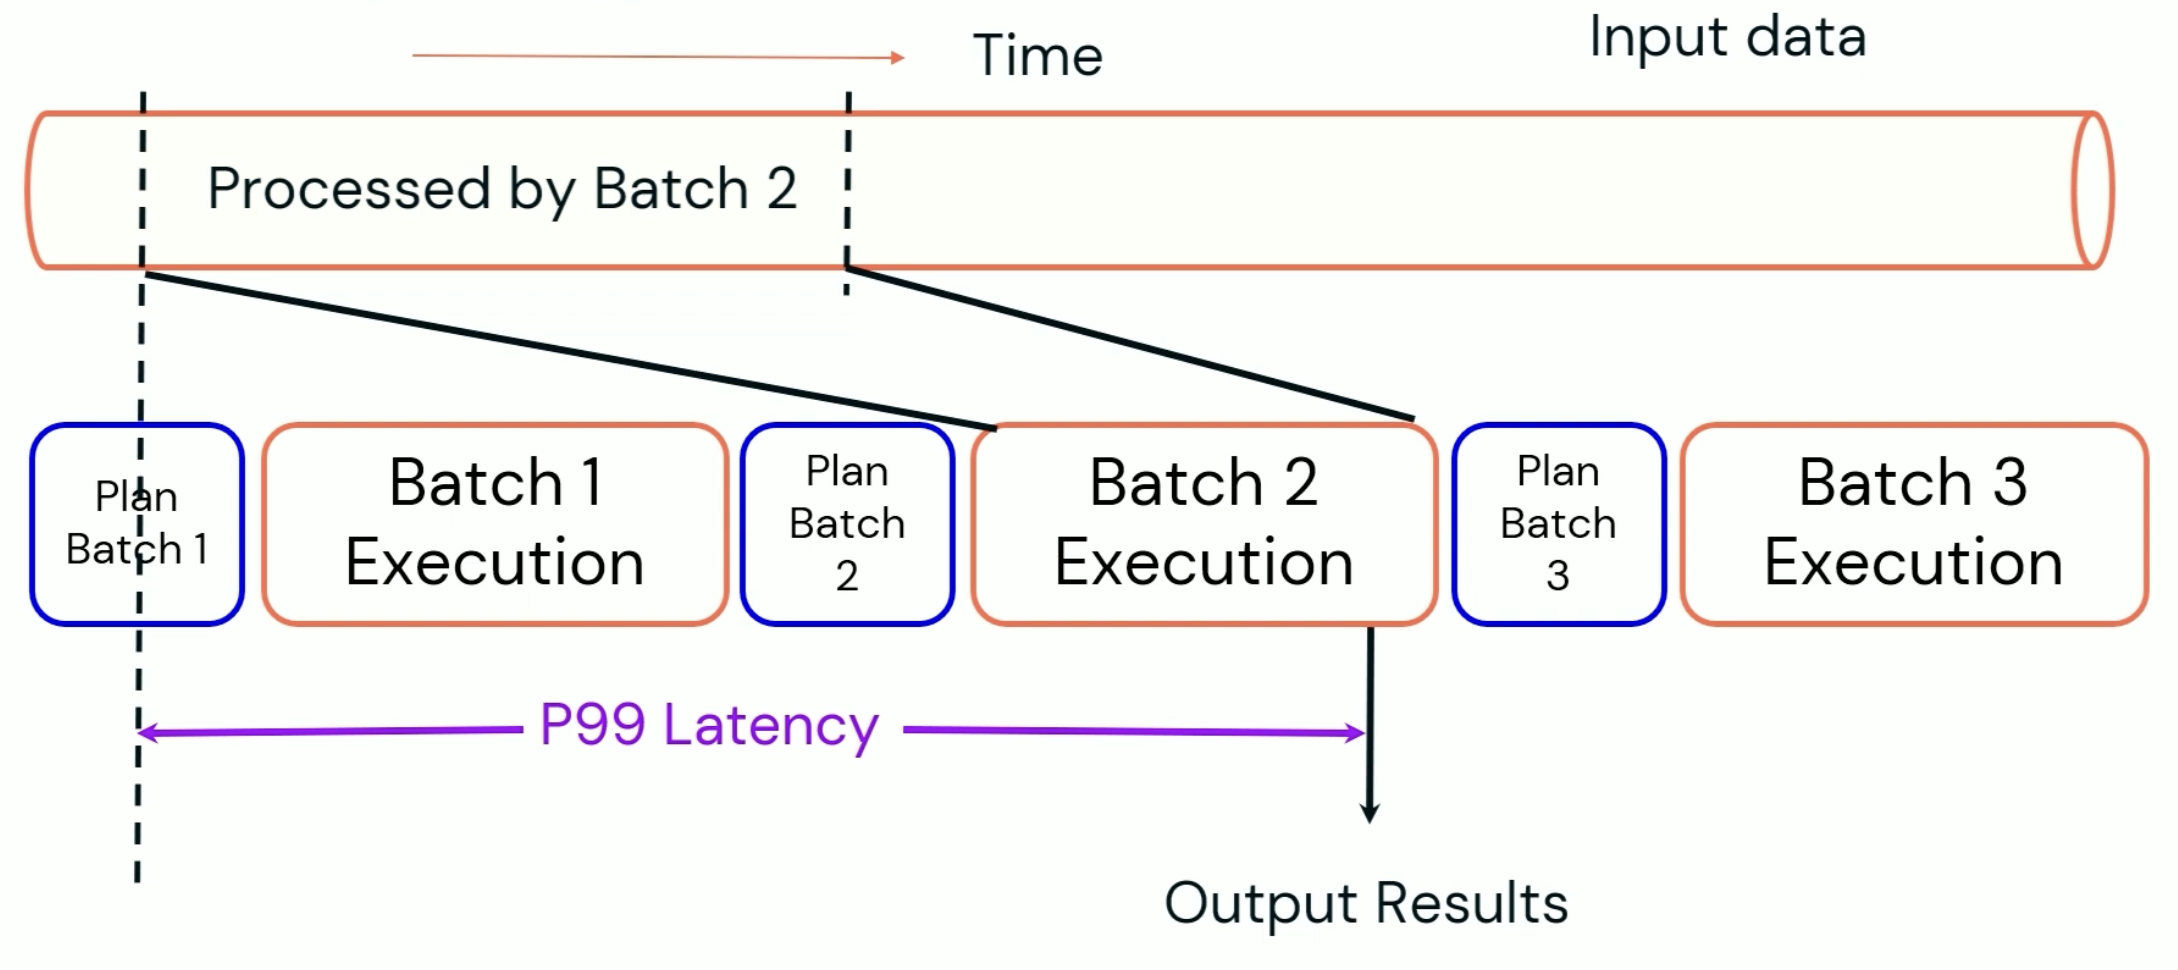
\includegraphics[width=0.88\textwidth]{image/engine/spark_micro_batch_latency.png}
  \caption{End-to-end latency profile in micro-batch mode: the trigger interval sets the latency floor.}
  \label{fig:spark-microbatch-latency}
\end{figure}

The trigger interval is the primary latency knob: shorter intervals lower latency but increase
scheduling overhead and reduce throughput per batch.
In practice, sub-100\,ms end-to-end latency is not achievable in this mode.

\subsubsection{Real-time Mode (Continuous Mode) — New in Spark 4}

\begin{figure}[H]
  \centering
  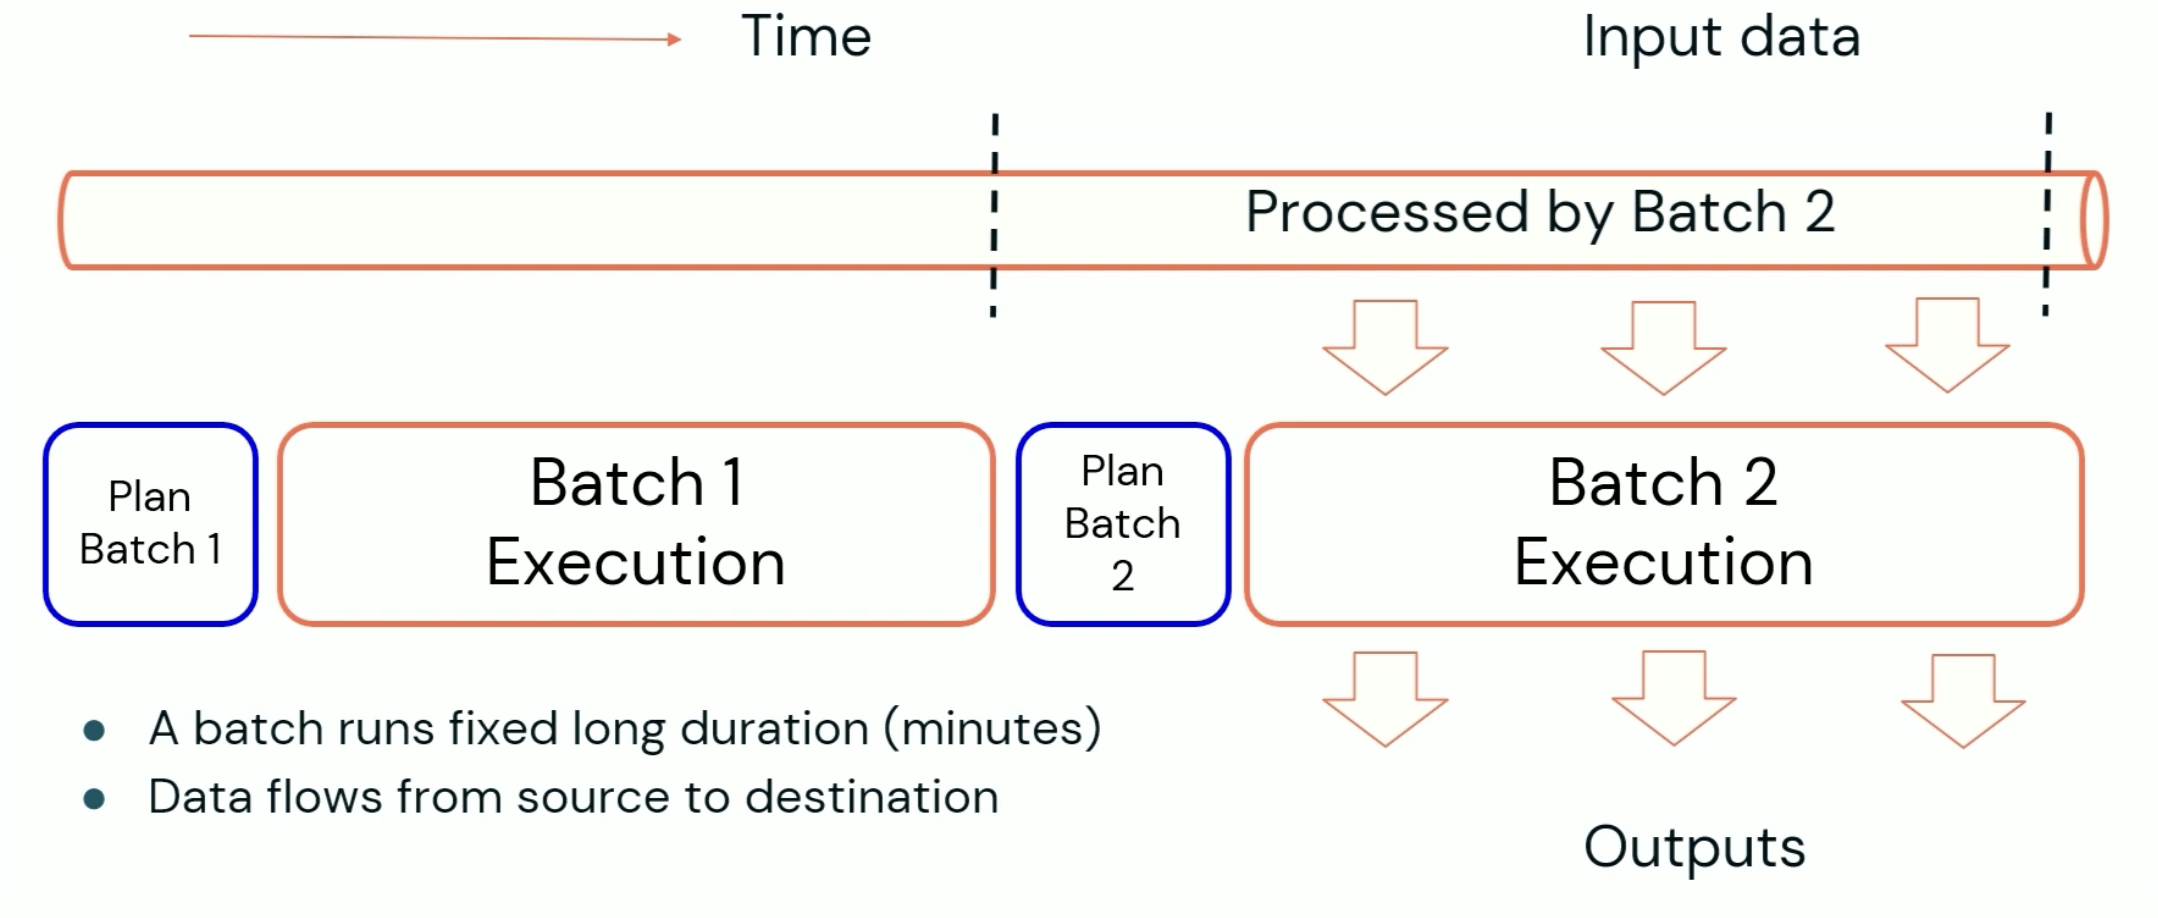
\includegraphics[width=0.88\textwidth]{image/engine/spark_rtm.png}
  \caption{Spark Real-time Mode: data streams continuously through the operator pipeline within a long-running batch window.}
  \label{fig:spark-rtm}
\end{figure}

\textbf{Real-time Mode} (also referred to as Continuous Mode) is a new execution mode
introduced in \textbf{Spark 4 / Databricks Runtime}, announced at the Data + AI Summit.
Rather than shrinking the micro-batch interval to reduce latency, it takes the opposite approach:
batches run for a \emph{long fixed window} (default 5 minutes),
but data flows \emph{continuously} through the operator pipeline
inside that window — never buffered to the batch boundary.

The fundamental changes made to the Spark runtime to enable this:

\begin{enumerate}
  \item \textbf{Concurrent stage scheduling} —
        in micro-batch mode, stages execute \emph{sequentially} (stage $n$ starts only after stage $n-1$ finishes).
        In real-time mode, all stages are scheduled \emph{concurrently} from the start of the batch window,
        so a record flows from source to sink without waiting for upstream stages to complete a full sweep.

  \item \textbf{Fresh source reads} —
        instead of reading a fixed offset range determined at the start of each batch,
        the source operator reads the \emph{most recent available data} continuously as it arrives,
        ensuring records enter the pipeline with minimal ingestion delay.

  \item \textbf{Streaming shuffle} —
        the shuffle layer (data exchange between stages) is redesigned to forward records immediately
        as they are produced, rather than materialising a full shuffle file at the end of a stage.
        This eliminates the per-stage synchronisation barrier that adds latency in micro-batch mode.

  \item \textbf{Operator-level streaming} —
        aggregation and stateful operators (including the new \texttt{TransformWithState} API)
        are modified to emit results incrementally as records arrive,
        rather than flushing outputs only at the end of each stage.

  \item \textbf{Incremental state cleanup} —
        instead of scanning the entire state store at the end of every batch,
        state expiry is spread across the full batch window —
        a few state-store rows are checked after every processed record,
        keeping per-record latency flat regardless of state store size.
\end{enumerate}

\begin{figure}[H]
  \centering
  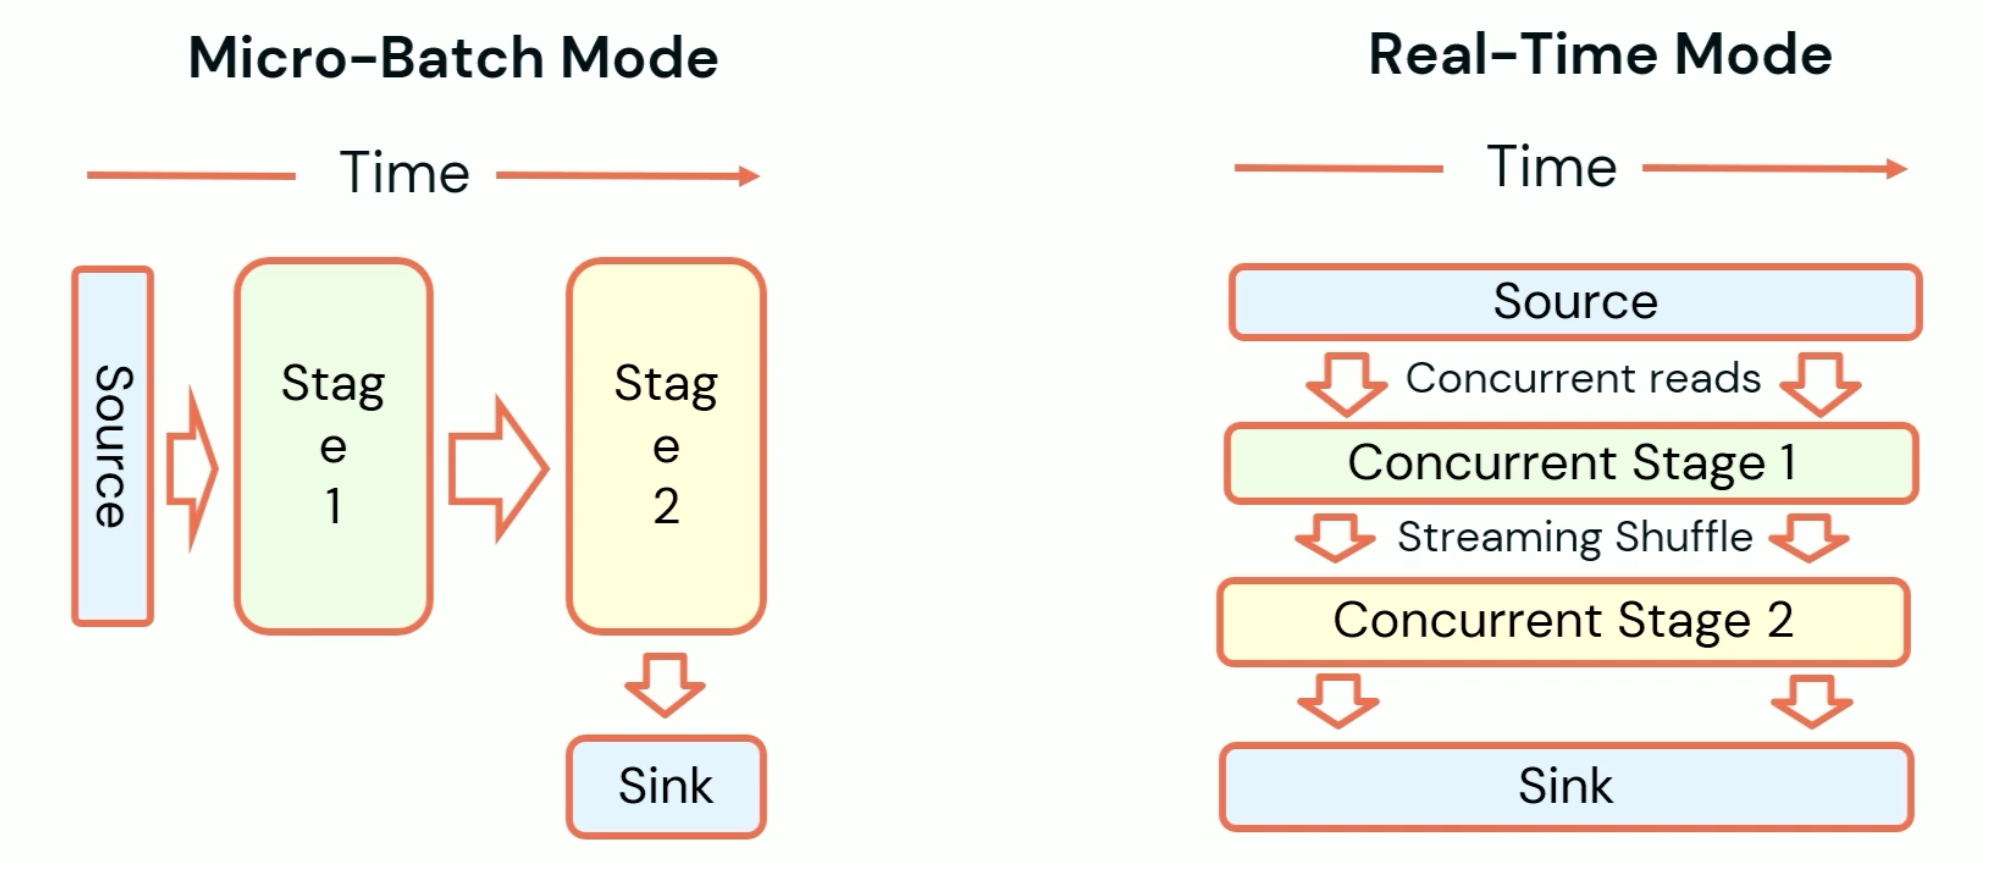
\includegraphics[width=0.65\textwidth]{image/engine/spark_rtm_change_1.png}
  \caption{Enabling real-time mode requires only a trigger change — the rest of the query is unchanged.}
  \label{fig:spark-rtm-change1}
\end{figure}

\begin{figure}[H]
  \centering
  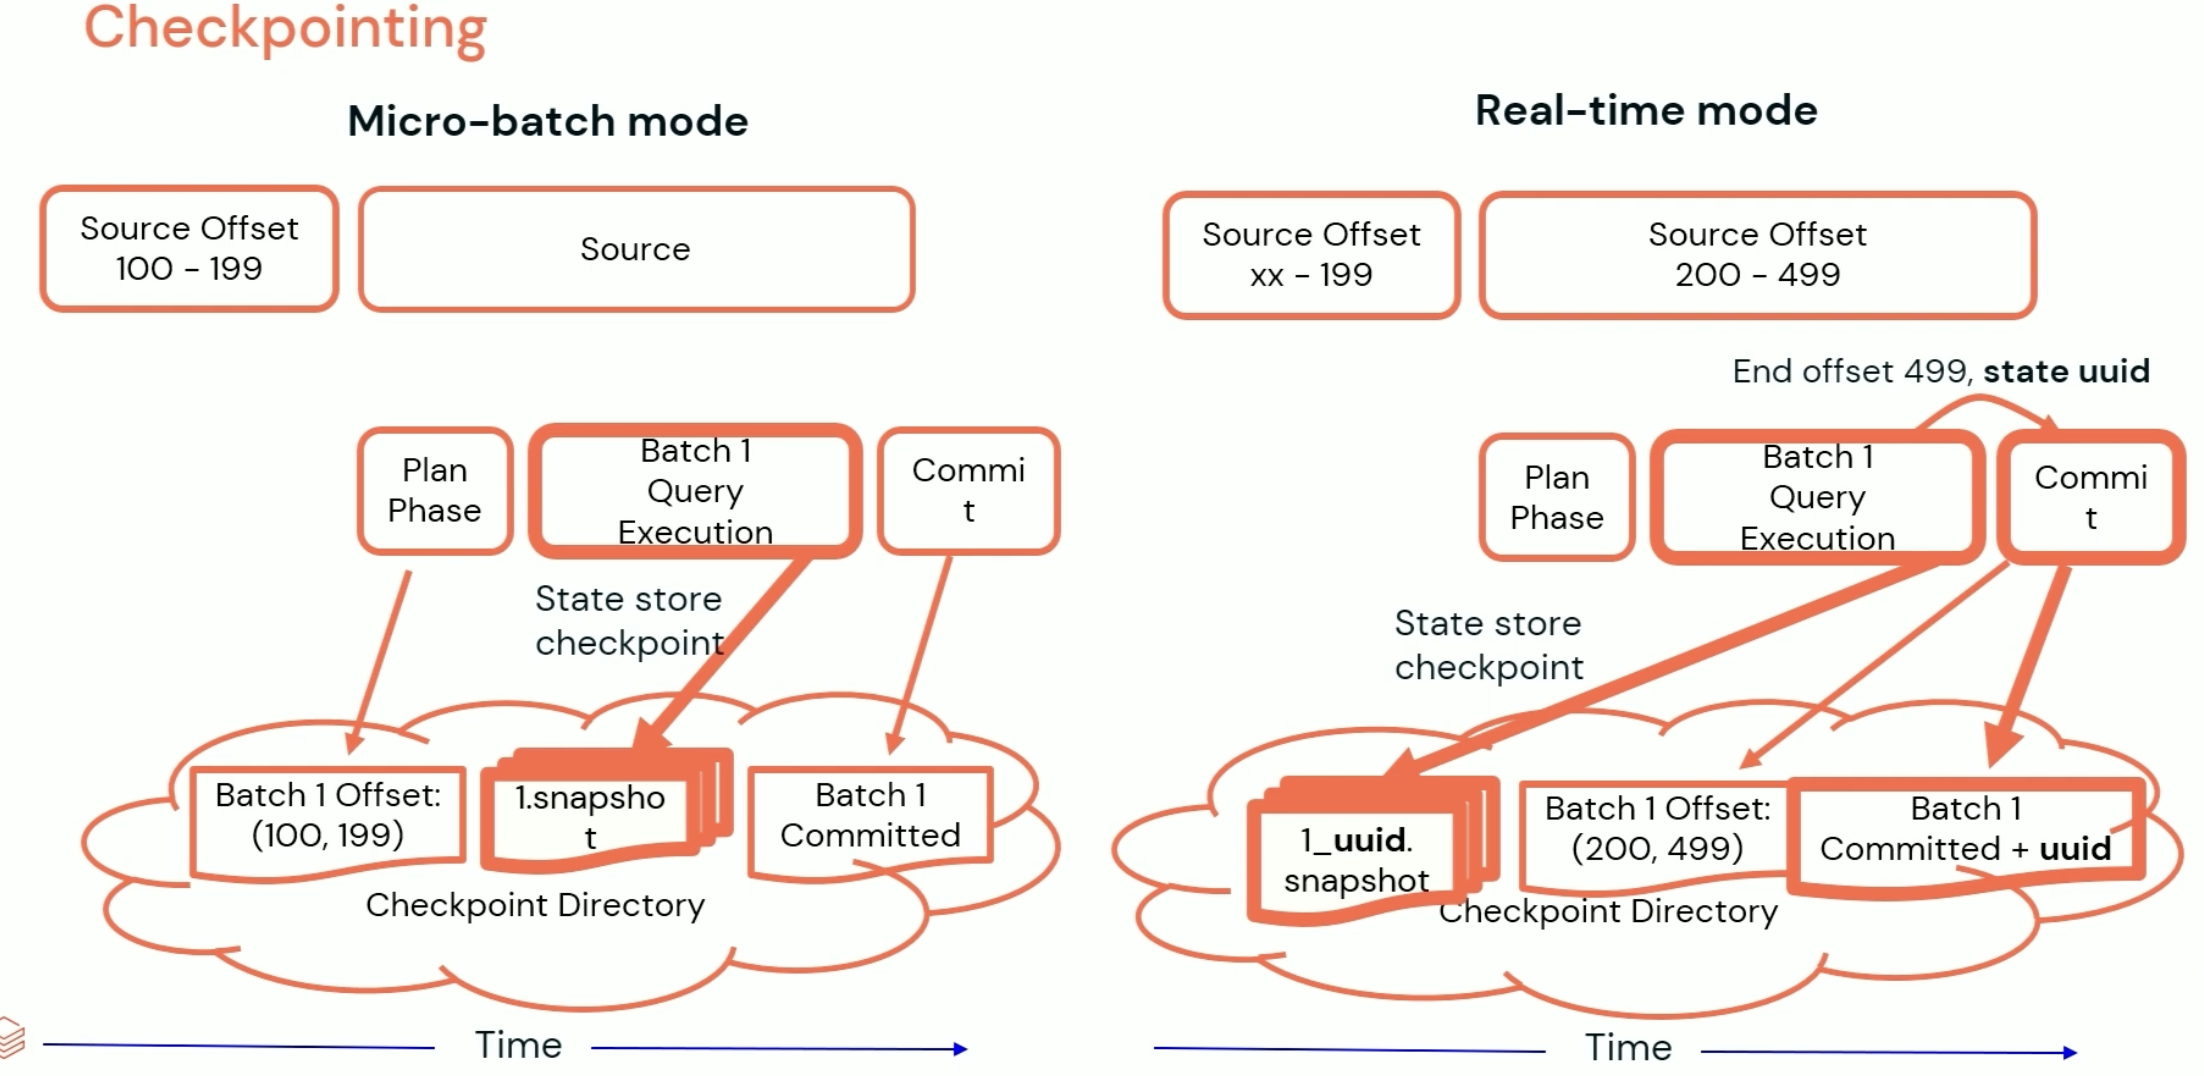
\includegraphics[width=0.65\textwidth]{image/engine/spark_rtm_change_2.png}
  \caption{Internal execution: stages run concurrently and records stream through without batch-end buffering.}
  \label{fig:spark-rtm-change2}
\end{figure}

\textbf{Checkpointing v2} is introduced alongside real-time mode.
In micro-batch mode, offsets are written to the checkpoint log at the \emph{beginning} of each batch,
making each batch idempotent on replay.
In real-time mode, the end offset is unknown until the batch window closes,
so offsets are written at the \emph{end} of the window together with a \textbf{globally unique ID}
recorded in the commit log.
This ID ties the offset commit to the state-store snapshot, eliminating ambiguity during recovery.
Checkpoint v2 also benefits micro-batch mode and will become the default in a future release.

\textbf{Processing semantics:}
\begin{itemize}
  \item \textbf{Exactly-once processing} — the same guarantee as micro-batch mode is maintained:
        each input record affects the final output exactly once.
  \item \textbf{End-to-end exactly-once} — depends on the sink; Kafka is natively supported.
        Custom sinks can implement idempotent writes via the \texttt{ForeachBatch} or Data Source V2 APIs.
  \item \textbf{Target latency} — sub-100\,ms (double-digit milliseconds in benchmarks),
        a \textbf{two orders of magnitude} improvement over the processing-time trigger.
  \item \textbf{Stateful operators supported} — aggregations, \texttt{TransformWithState}, and other
        stateful operations work in real-time mode (unlike the old Spark 2.3 Continuous Processing experiment).
\end{itemize}

\begin{tcolorbox}[colback=NavyBlue!6, colframe=NavyBlue, title=\textbf{Availability}]
Real-time Mode is currently in \textbf{public preview} on Databricks Runtime and is approved
by the Spark PMC for open-sourcing.
It will be available in the Apache Spark open-source release in a future version.
To try it today, contact your Databricks account team.
\end{tcolorbox}

\subsection{Mechanisms in Spark Streaming}

\subsubsection{How Data is Processed}

\begin{table}[H]
  \centering
  \caption{Data processing comparison: micro-batch vs.\ real-time mode.}
  \label{tab:spark-processing}
  \begin{tabularx}{\textwidth}{lXX}
    \toprule
    \textbf{Aspect}        & \textbf{Micro-batch}                           & \textbf{Real-time Mode (Spark 4 / Databricks)} \\
    \midrule
    Execution unit         & Bounded DataFrame per trigger interval         & Long batch window (default 5 min); data streams continuously inside \\
    Stage scheduling       & Sequential — stage $n$ waits for $n-1$         & Concurrent — all stages active simultaneously \\
    Shuffle                & Materialised at stage boundary                 & Streaming shuffle — records forwarded immediately \\
    Latency                & 100\,ms – seconds (bounded by trigger)         & Sub-100\,ms (double-digit ms in benchmarks) \\
    Offset commit          & At \emph{beginning} of batch (idempotent)      & At \emph{end} of batch with globally unique ID (Checkpoint v2) \\
    Supported operators    & Full (aggregations, joins, stateful)           & Full, incl.\ \texttt{TransformWithState} \\
    Exactly-once           & Yes, with idempotent / transactional sinks     & Yes — same guarantee as micro-batch \\
    Availability           & Stable, open source                            & Public preview (Databricks); open-source pending \\
    \bottomrule
  \end{tabularx}
\end{table}

\subsubsection{Checkpointing}

Spark's checkpointing mechanism ensures that a streaming query can recover from any failure
without replaying the entire history of events.
Two types of data are persisted to a reliable, user-specified checkpoint directory (HDFS, S3, or local):

\begin{itemize}
  \item \textbf{Offset log} — a write-ahead log (WAL) that records the source offsets consumed in
        each micro-batch. On restart, Spark reads the WAL to determine exactly where to resume,
        ensuring no record is skipped.
  \item \textbf{State store snapshots} — for stateful queries (aggregations, joins), periodic snapshots
        of the in-memory or RocksDB key-value state are flushed to the checkpoint directory.
        On recovery, the state is restored from the latest snapshot rather than being recomputed from scratch.
\end{itemize}

\begin{lstlisting}[language=Python, caption={Setting the checkpoint location in Spark.}]
stream.writeStream \
    .option("checkpointLocation", "/tmp/checkpoints/my_query") \
    .trigger(processingTime="5 seconds") \
    .start()
\end{lstlisting}

\subsubsection{State Storage}

Stateful streaming operations (windowed aggregations, deduplication, stream–stream joins)
require maintaining keyed state across micro-batches.
Spark offers two pluggable state store backends:

\begin{itemize}
  \item \textbf{HDFSBackedStateStore (in-memory)} — state is stored in the JVM heap of each executor.
        Snapshots are periodically serialised and written to the checkpoint path on HDFS or S3.
        Fast for small-to-medium state, but bounded by executor heap size; large state triggers GC pauses.
  \item \textbf{RocksDBStateStore} (Spark 3.2+) — state is kept on local SSD via RocksDB.
        Supports state sizes far exceeding available heap with no GC pressure.
        Snapshots are uploaded incrementally to the checkpoint store, reducing checkpoint cost for large state.
\end{itemize}

\subsubsection{Fault Tolerance}

\begin{itemize}
  \item \textbf{Executor failure} — the Driver reschedules the failed task on another Executor.
        Because offsets are not committed until the micro-batch completes successfully,
        the retry reads the same records, guaranteeing at-least-once processing.
        Combined with an idempotent or transactional sink, this achieves exactly-once semantics.
  \item \textbf{Driver failure} — the query is restarted from the checkpoint.
        The offset log tells it exactly where to resume; state snapshots restore aggregation state,
        avoiding a full replay of the event history.
  \item \textbf{Source requirement} — the source must support offset-based re-reads (Kafka, Delta Lake, files).
        Non-replayable sources (TCP sockets, stdin) cannot provide recovery guarantees.
\end{itemize}

\subsubsection{Pros and Cons}

\begin{itemize}
  \item[\textbf{+}] Unified API — identical DataFrame/SQL code for batch and streaming jobs, drastically reducing the engineering surface area.
  \item[\textbf{+}] Full stateful operator suite in micro-batch mode: aggregations, time-window joins, deduplication, arbitrary stateful functions.
  \item[\textbf{+}] Extremely large ecosystem — Delta Lake, MLlib, Spark Connect, Spark SQL, broad connector library, mature tooling.
  \item[\textbf{+}] Production-hardened and widely deployed across all major cloud providers.
  \item[\textbf{--}] Micro-batch latency floor — sub-100\,ms end-to-end latency is not achievable in the default mode.
  \item[\textbf{+}] Real-time Mode (Spark 4) achieves sub-100\,ms latency with exactly-once semantics and full stateful operator support — closing the gap with purpose-built streaming engines like Flink.
  \item[\textbf{--}] Real-time Mode is currently in public preview (Databricks only); not yet available in open-source Spark.
  \item[\textbf{--}] Very large keyed state can induce JVM GC pressure (partially mitigated with the RocksDB backend).
\end{itemize}

\subsubsection{Suitable Applications}

\begin{itemize}
  \item \textbf{Micro-batch} — streaming ETL into data warehouses, fraud detection aggregations, real-time dashboards where second-level freshness is acceptable, and any workload already using Spark for batch that needs to add a streaming layer.
  \item \textbf{Real-time mode} — simple event routing, payload transformation, or enrichment pipelines where millisecond latency is needed but stateful logic is not required.
  \item \textbf{Not ideal for} — complex event processing (CEP), sub-millisecond SLAs, very large continuously-growing keyed state, or workloads requiring native exactly-once end-to-end without idempotent sinks.
\end{itemize}
